\begin{figure}[!h]
\centering
\resizebox{\columnwidth}{!}{


\tikzset{every picture/.style={line width=0.75pt}} %set default line width to 0.75pt        

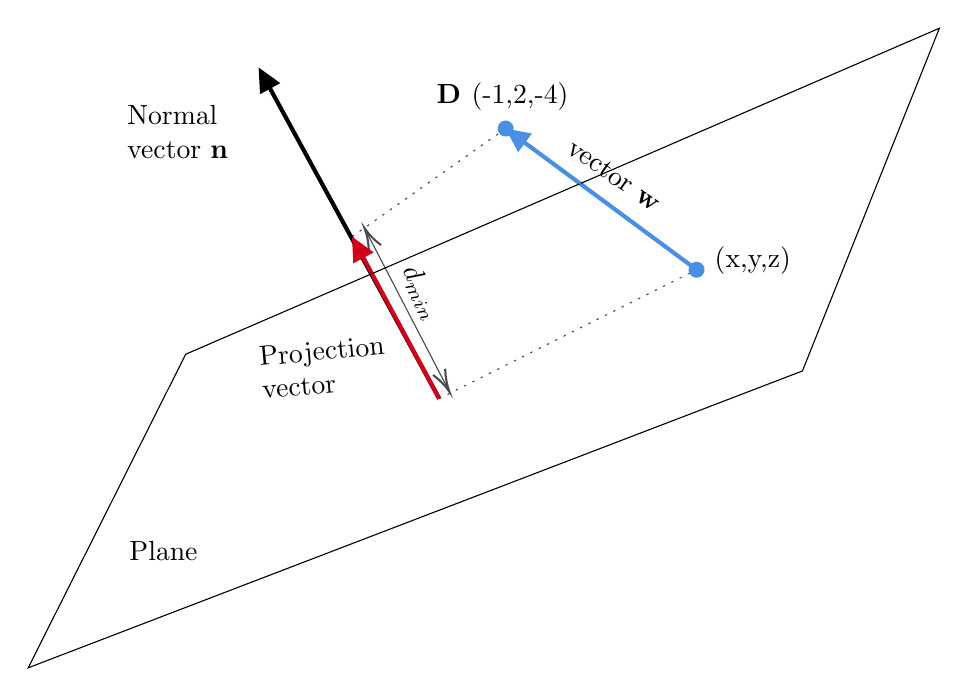
\begin{tikzpicture}[x=0.75pt,y=0.75pt,yscale=-1,xscale=1]
%uncomment if require: \path (0,324); %set diagram left start at 0, and has height of 324

%Straight Lines [id:da012474511036709712] 
\draw [color={rgb, 255:red, 74; green, 74; blue, 74 }  ,draw opacity=1 ] [dash pattern={on 0.84pt off 2.51pt}]  (165.51,108.36) -- (239.51,56.27) ;
%Straight Lines [id:da164610693713777] 
\draw [color={rgb, 255:red, 74; green, 74; blue, 74 }  ,draw opacity=1 ] [dash pattern={on 0.84pt off 2.51pt}]  (207.51,186.36) -- (331.51,124.27) ;
%Straight Lines [id:da0009900971082483778] 
\draw [color={rgb, 255:red, 74; green, 74; blue, 74 }  ,draw opacity=1 ]   (211.58,181.43) -- (172.42,105.98) ;
\draw [shift={(171.5,104.2)}, rotate = 422.57] [color={rgb, 255:red, 74; green, 74; blue, 74 }  ,draw opacity=1 ][line width=0.75]    (10.93,-3.29) .. controls (6.95,-1.4) and (3.31,-0.3) .. (0,0) .. controls (3.31,0.3) and (6.95,1.4) .. (10.93,3.29)   ;
\draw [shift={(212.5,183.2)}, rotate = 242.57] [color={rgb, 255:red, 74; green, 74; blue, 74 }  ,draw opacity=1 ][line width=0.75]    (10.93,-3.29) .. controls (6.95,-1.4) and (3.31,-0.3) .. (0,0) .. controls (3.31,0.3) and (6.95,1.4) .. (10.93,3.29)   ;
%Straight Lines [id:da6317108471264852] 
\draw [line width=1.5]    (207.51,186.36) -- (122.42,30.38) ;
\draw [shift={(120.51,26.87)}, rotate = 421.39] [fill={rgb, 255:red, 0; green, 0; blue, 0 }  ][line width=0.08]  [draw opacity=0] (11.61,-5.58) -- (0,0) -- (11.61,5.58) -- cycle    ;
%Straight Lines [id:da4711513779445873] 
\draw [color={rgb, 255:red, 74; green, 144; blue, 226 }  ,draw opacity=1 ][line width=1.5]    (331.51,124.27) -- (242.72,58.64) ;
\draw [shift={(239.51,56.27)}, rotate = 396.47] [fill={rgb, 255:red, 74; green, 144; blue, 226 }  ,fill opacity=1 ][line width=0.08]  [draw opacity=0] (11.61,-5.58) -- (0,0) -- (11.61,5.58) -- cycle    ;
%Straight Lines [id:da281513313013386] 
\draw [color={rgb, 255:red, 208; green, 2; blue, 27 }  ,draw opacity=1 ][line width=1.5]    (207.51,186.36) -- (167.4,111.89) ;
\draw [shift={(165.51,108.36)}, rotate = 421.7] [fill={rgb, 255:red, 208; green, 2; blue, 27 }  ,fill opacity=1 ][line width=0.08]  [draw opacity=0] (11.61,-5.58) -- (0,0) -- (11.61,5.58) -- cycle    ;
%Shape: Polygon [id:ds23253650680866844] 
\draw   (85.38,164.99) -- (448.5,7.93) -- (382.5,173.07) -- (9.5,316.07) -- (9.5,316.07) -- cycle ;
%Straight Lines [id:da02842289374539675] 
\draw [color={rgb, 255:red, 74; green, 144; blue, 226 }  ,draw opacity=1 ]   (239.51,56.27) -- (331.51,124.27) ;
\draw [shift={(331.51,124.27)}, rotate = 36.47] [color={rgb, 255:red, 74; green, 144; blue, 226 }  ,draw opacity=1 ][fill={rgb, 255:red, 74; green, 144; blue, 226 }  ,fill opacity=1 ][line width=0.75]      (0, 0) circle [x radius= 3.35, y radius= 3.35]   ;
\draw [shift={(239.51,56.27)}, rotate = 36.47] [color={rgb, 255:red, 74; green, 144; blue, 226 }  ,draw opacity=1 ][fill={rgb, 255:red, 74; green, 144; blue, 226 }  ,fill opacity=1 ][line width=0.75]      (0, 0) circle [x radius= 3.35, y radius= 3.35]   ;

% Text Node
\draw (56,44) node [anchor=north west][inner sep=0.75pt]   [align=left] {Normal \\vector \textbf{n} };
% Text Node
\draw (118.97,160.37) node [anchor=north west][inner sep=0.75pt]  [rotate=-354.79] [align=left] {Projection \\vector};
% Text Node
\draw (205,33) node [anchor=north west][inner sep=0.75pt]   [align=left] {\textbf{D }(-1,2,-4)};
% Text Node
\draw (339,112) node [anchor=north west][inner sep=0.75pt]   [align=left] {(x,y,z)};
% Text Node
\draw (272.66,59.12) node [anchor=north west][inner sep=0.75pt]  [rotate=-34.52] [align=left] {vector \textbf{w} };
% Text Node
\draw (198.69,119.24) node [anchor=north west][inner sep=0.75pt]  [rotate=-64.65] [align=left] {$d_{min}$};
% Text Node
\draw (57,254.07) node [anchor=north west][inner sep=0.75pt]   [align=left] {Plane};


\end{tikzpicture}
}
\caption{Right Angled Triangle by Latex-Tikz}
\label{myfig:solutions/1/7/}
\end{figure}
In $\triangle{ABC}$, $\vec{M}$ is midpoint of $\vec{AB}$ and $\vec{MD}$ is parallel to $\vec{BC}$, hence,
\begin{align}
&\vec{M} = \frac{\vec{A}+\vec{B}}{2}\label{eq:solutions/1/7/1}\\
&\vec{MD} \parallel \vec{BC}\label{eq:solutions/1/7/2}
\end{align}
Let $\vec{m_M_D}$ and $\vec{m_B_C}$ are direction vectors of $\vec{MD}$ and $\vec{BC}$ respectively. Then,
\begin{align}
\vec{m_M_D} &= \vec{M} - \vec{D} = \frac{\vec{A}+\vec{B}}{2} - \vec{D}\\
\vec{m_B_C} &= \vec{B} - \vec{C}
\end{align}
Now from \eqref{eq:solutions/1/7/2} we get,
\begin{align}
\vec{m_M_D} &= k\vec{m_B_C}\\
\implies\frac{\vec{A}+\vec{B}}{2} - \vec{D} &= k(\vec{B} - \vec{C})\label{eq:solutions/1/7/New1}
\end{align}
Let $\vec{D}$ = $\frac{m\vec{A}+\vec{C}}{m+1}$, then from \eqref{eq:solutions/1/7/New1} we get,
\begin{align}
\frac{\vec{A}+\vec{B}}{2} - \frac{m\vec{A}+\vec{C}}{m+1} = k(\vec{B} - \vec{C})
\end{align}
\begin{align}
\implies\brak{\frac{1}{2}-\frac{m}{m+1}}\vec{A}+\brak{\frac{1}{2}-k}\vec{B}+\brak{k-\frac{1}{m+1}}\vec{C} =0
\end{align}
Since $\vec{A}$, $\vec{B}$ and $\vec{C}$ are linearly dependent as they form $\triangle{ABC}$ then 
\begin{align}
\frac{1}{2}-\frac{m}{m+1} &= 0\label{solve1}\\
\frac{1}{2}-k & = 0\label{solve2}\\
k-\frac{1}{m+1} &= 0\label{solve3}
\end{align}
Solving \eqref{solve1}, \eqref{solve2} and \eqref{solve3} we get $k=\frac{1}{2}$ and $m = 1$. Hence, substituting value of $m$ in $\vec{D}$ we get,
\begin{align}
&\vec{D} = \frac{\vec{A}+\vec{C}}{2}\label{eq:solutions/1/7/3}
\end{align}
Hence Proved.\\
From figure \ref{myfig:solutions/1/7/},
\begin{align}
(\vec{M}-\vec{D})(\vec{A}-\vec{D}) &=\brak{\frac{\vec{A}+\vec{B}}{2} - \frac{\vec{A}+\vec{C}}{2}}(\vec{A}-\vec{C})\\
\implies(\vec{M}-\vec{D})(\vec{A}-\vec{D}) &=\frac{1}{2}\brak{\vec{B}-\vec{C}}(\vec{A}-\vec{C})\\
\implies(\vec{M}-\vec{D})(\vec{A}-\vec{D}) &=0\label{eq:solutions/1/7/4}\quad{[$\because\vec{BC}\perp\vec{AC}$]}
\end{align}
From \eqref{eq:solutions/1/7/4}, it is proved that $\vec{MD}\perp\vec{AC}$\\
Again we get,
\begin{align}
\vec{C-M} &= \vec{C - D}+\vec{D - M}\\
\implies\vec{C-M} &= \vec{A - D}+\vec{D - M}\quad\text{[From \eqref{eq:solutions/1/7/3}]}\\
\implies\vec{C - M} &= \vec{A - M}\label{eq:solutions/1/7/Fin1}\\
\implies\vec{C - M} &= \vec{A} - \vec{\frac{\vec{A}+\vec{B}}{2}}\qquad\text{[From \eqref{eq:solutions/1/7/1}]}\\
\implies\vec{C - M} &= \frac{1}{2}(\vec{A-B})\\
\implies\norm{\vec{C - M}} &= \frac{1}{2}\norm{\vec{A-B}}\label{eq:solutions/1/7/Fin2}
\end{align}
Hence from \eqref{eq:solutions/1/7/Fin1} and \eqref{eq:solutions/1/7/Fin2} proved,\\ $\vec{CM}$ = $\vec{MA}$ = $\frac{1}{2}$ $\vec{AB}$
\end{document}
